\section{Traitement des images et création des matrices pour l'algorithme d'apprentissage}

\subsection{Présentation des images}

A chaque sujet correspond une image de dimension (182, 218, 182). Ce sont donc des images 3D qui sont regroupées en un seul volume. Le fichier image correspond donc a un volume 4D qui correspond aux dimensions d'une image plus le nombre de sujets.


\begin{figure}[htpb]
	\centering
	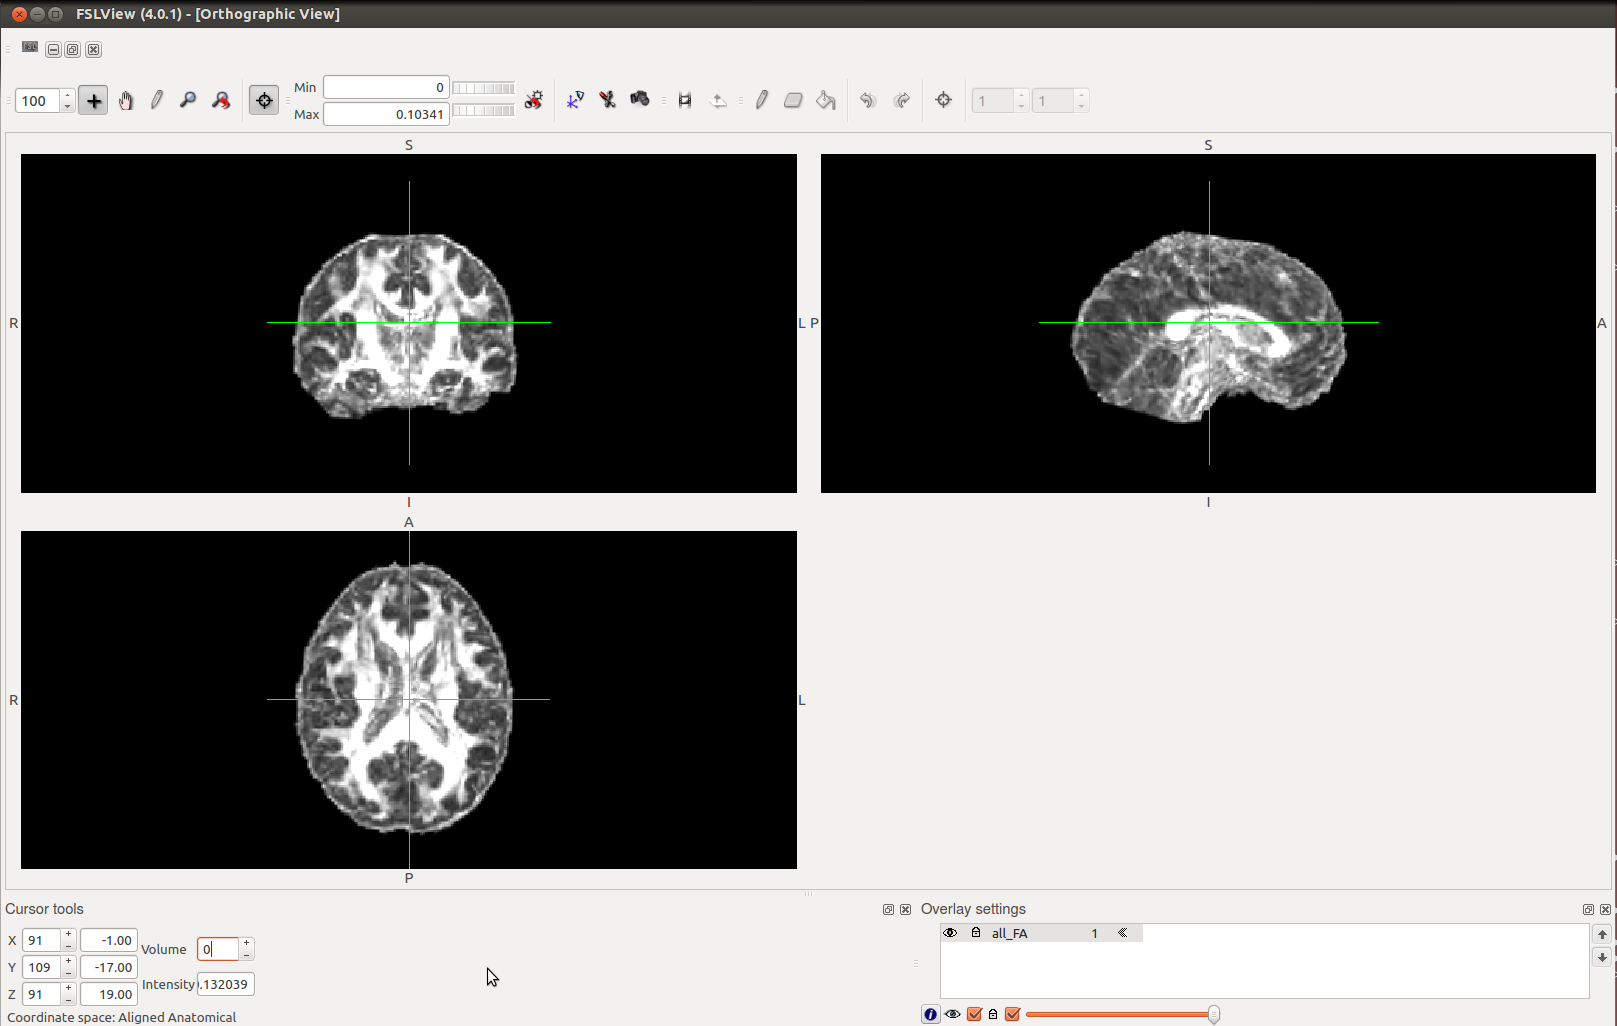
\includegraphics[scale = 0.5]{images/example_dwi}
	\caption{IRM de diffusion.}
	\label{fig:IRM}
\end{figure}

\begin{figure}[htpb]
	\centering
	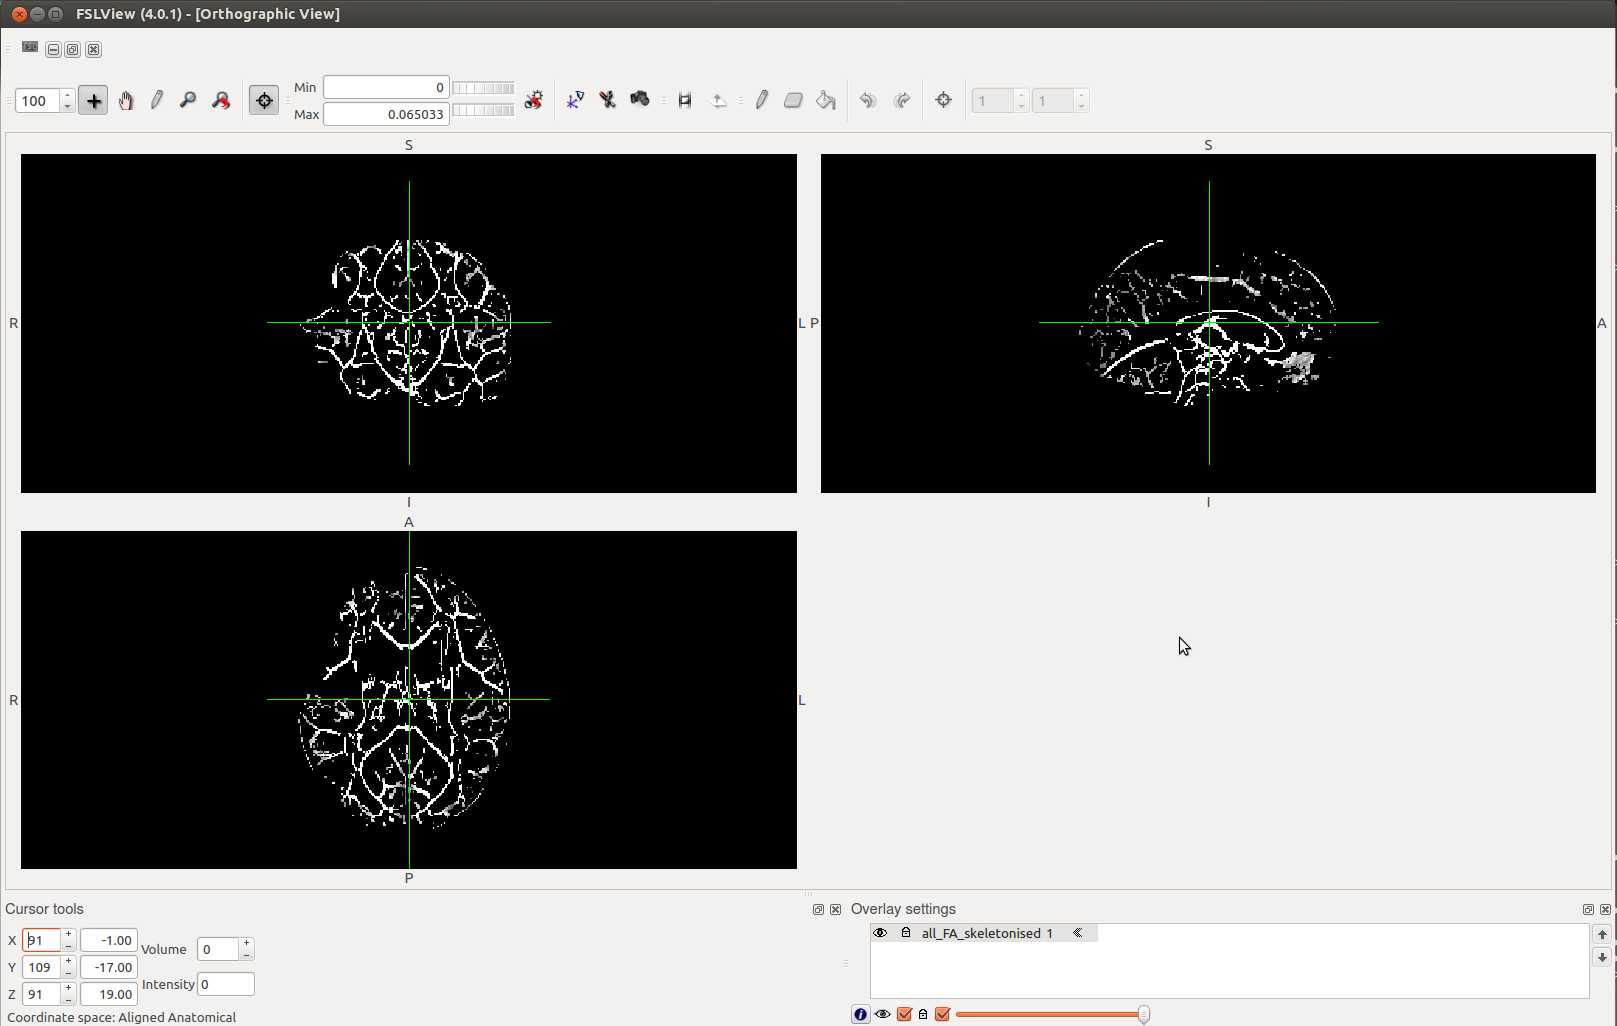
\includegraphics[scale = 0.5]{images/example_dwi_skel}
	\caption{IRM de diffusion squeletisé.}
	\label{fig:IRM_skel}
\end{figure}


\subsection{Création du masque}

Chaque image fait environ deux millions de voxels (pixel du cerveau). Nous allons appliquer un masque afin de réduire le nombre de voxel et ainsi focaliser notre analyse sur une plus petite partie du cerveau. Cela nous permettra d'éliminer une grande partie des voxels qui ne nous intéressent pas. 
Ce masque (voir~\autoref{fig:masque}) sera réalisé selon les images de base avec un certain seuil suivi d'un peaufinage basé sur un atlas qui va nous permettre de sélectionner des régions du cerveau qui ne sont pas révélatrices dans notre cas. 

Dans le cas des images squeletonisés(voir~\autoref{fig:masque squelétisé}), nous créons le masque sur la base de ces images. 

Dans le cas du masque tronqué (voir~\autoref{fig:mask tronqué}), nous suivons les mêmes étapes ci-dessus, suivi de l'élimination des zones du cerveau non informative (l'arrière du cerveau).



\begin{figure}[h]
	\centering
	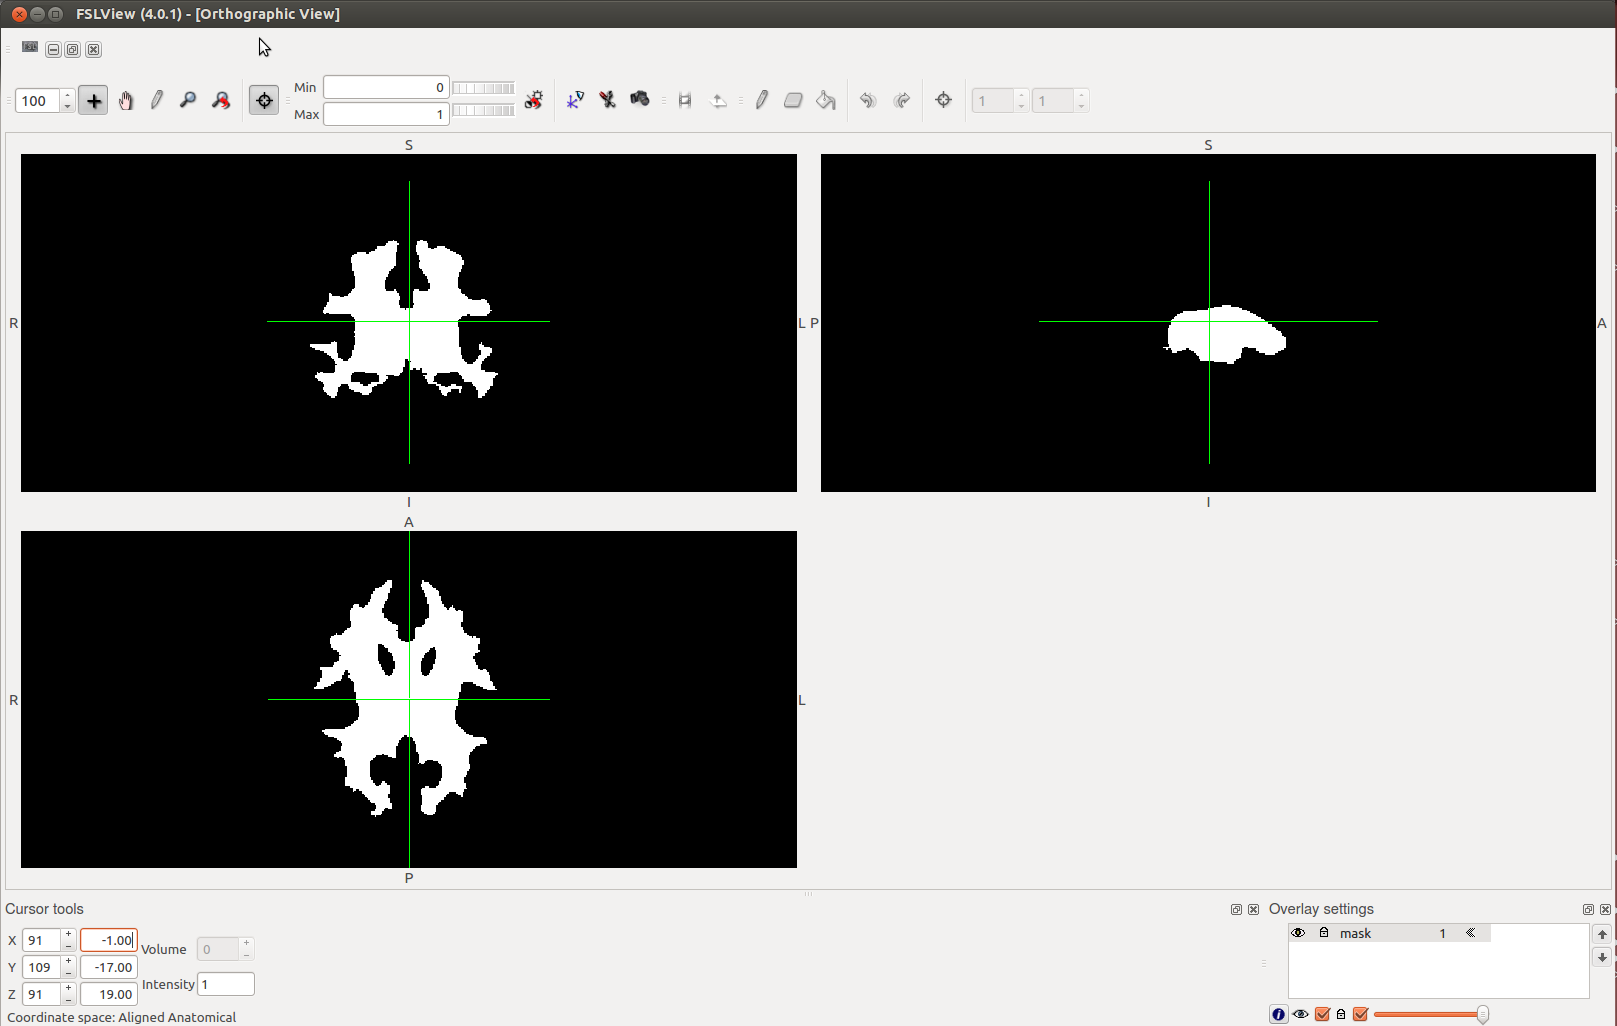
\includegraphics[scale = 0.5]{images/mask}
	\caption{Masque sans modification.}
	\label{fig:masque}
\end{figure}

\begin{figure}[h]
	\centering
	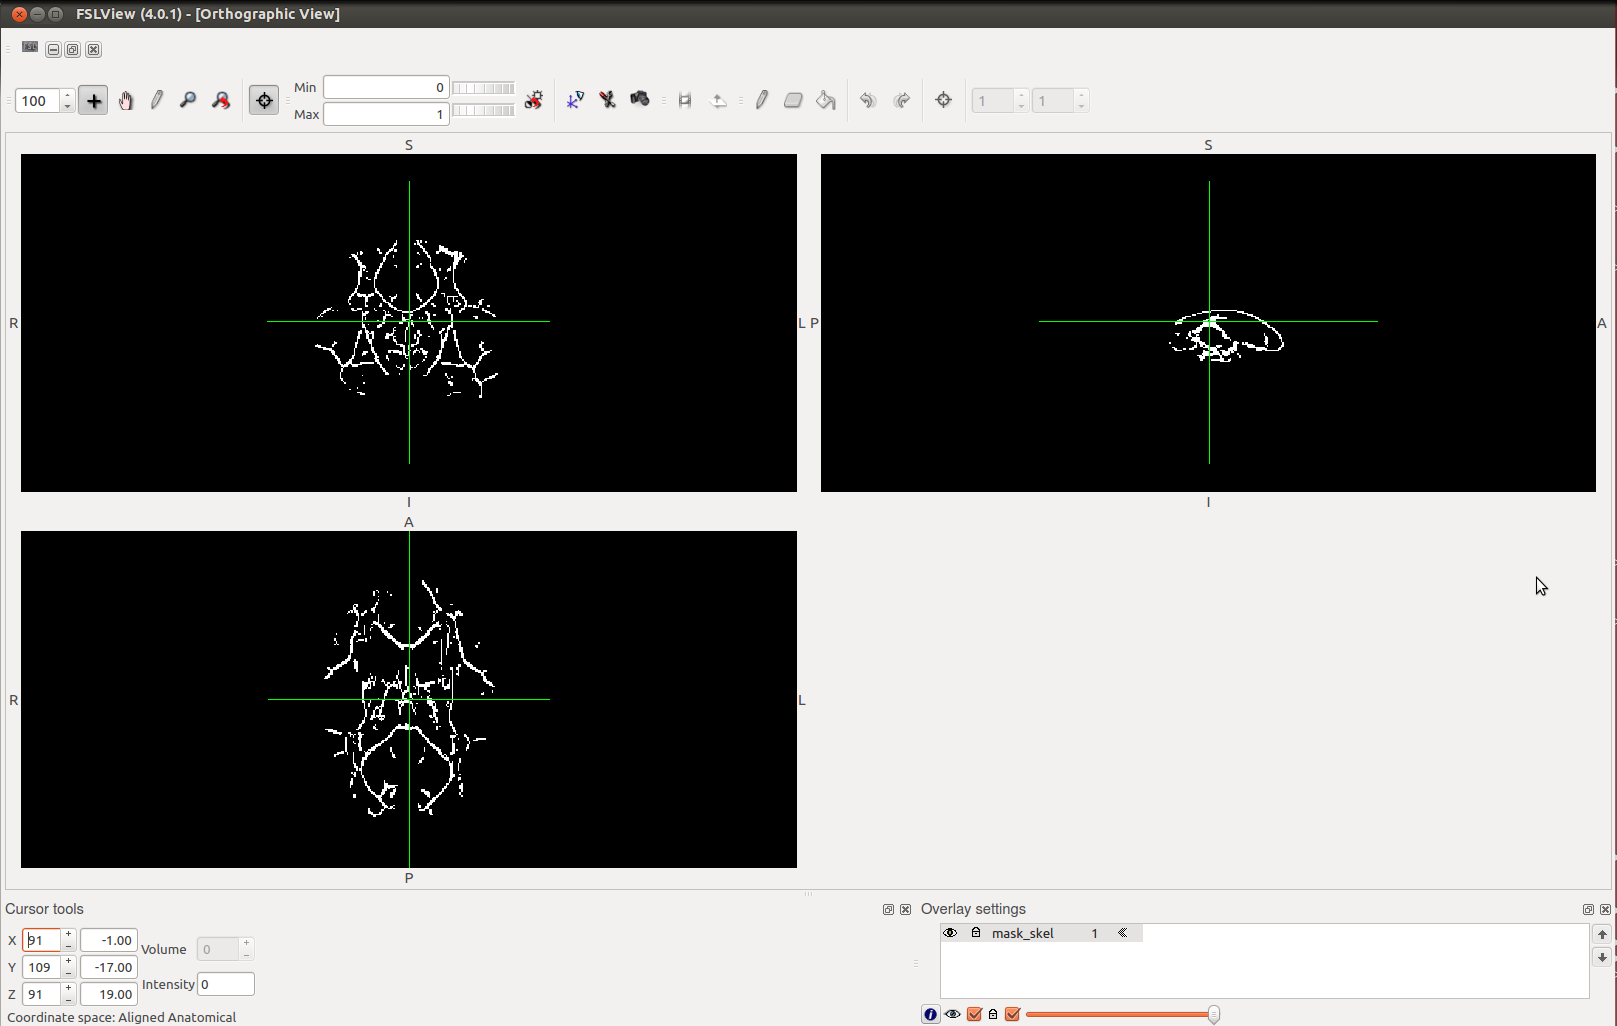
\includegraphics[scale = 0.5]{images/mask_skel}
	\caption{Masque réalisé à partir des images squelétisées.}
	\label{fig:masque squelétisé}
\end{figure}
  	
\begin{figure}[t]
	\centering
	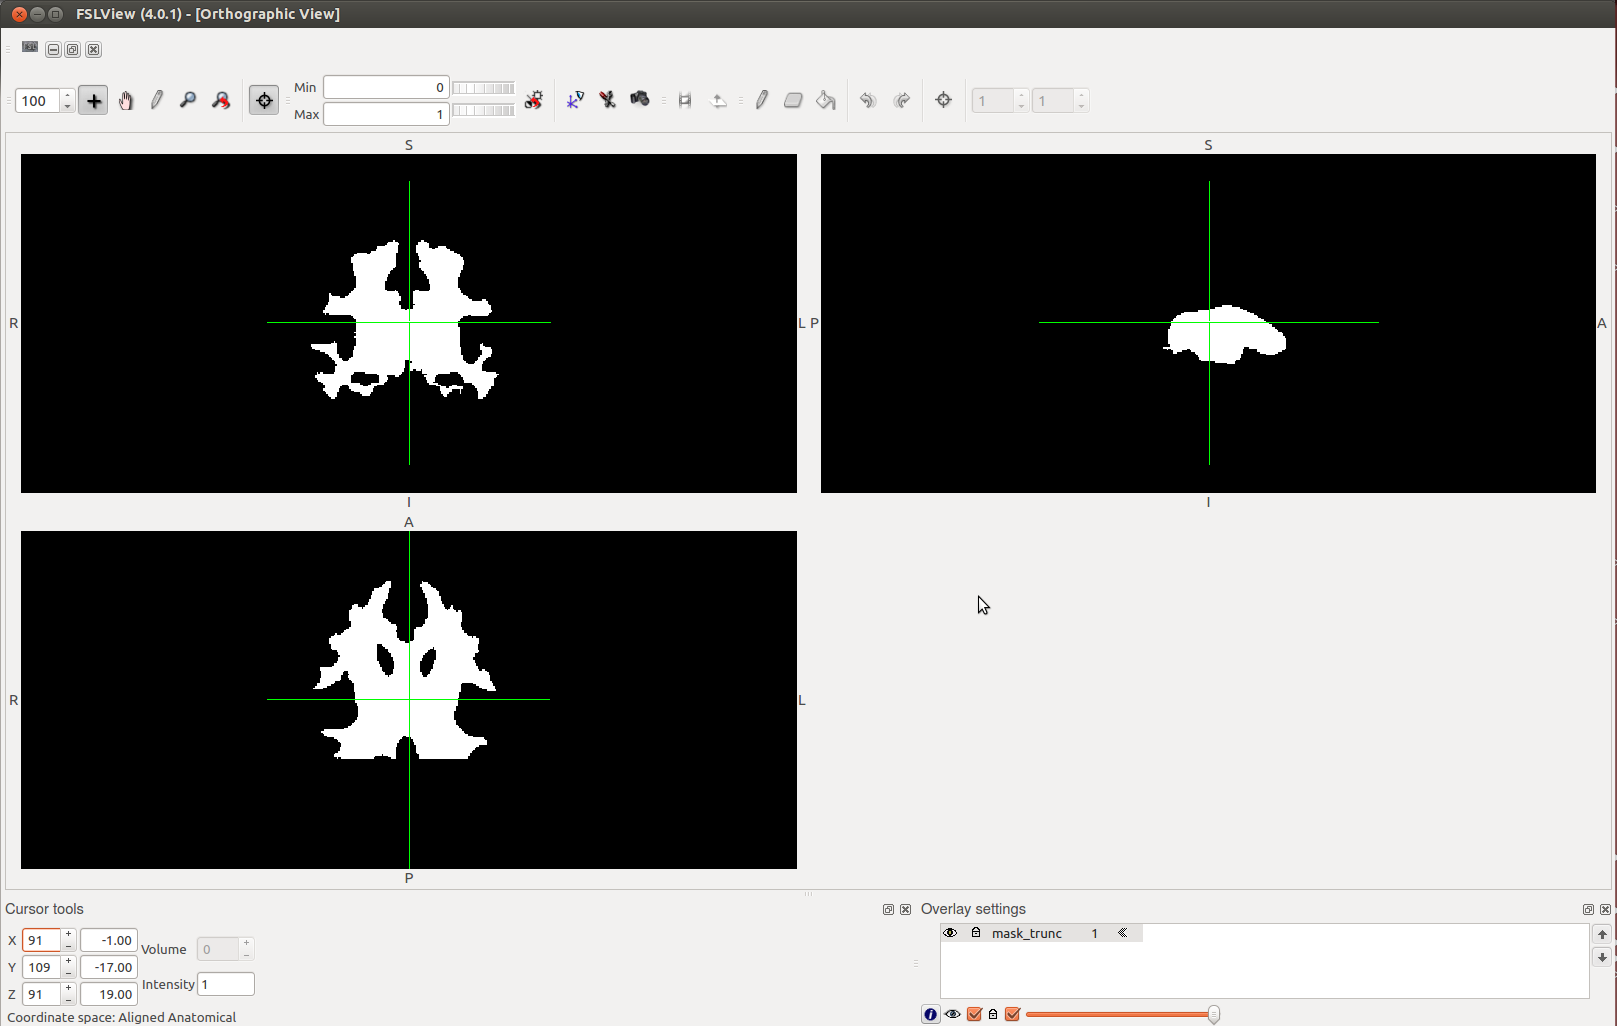
\includegraphics[scale = 0.5]{images/mask_trunk}
	\caption{Masque tronqué.}
	\label{fig:mask tronqué}
\end{figure}


\subsection{Application du masque}

Chaque image 3D sera transformée en un vecteur ligne. Celui-ci, que nous appellerons \textit{vecteur d'image} se verra appliqué le masque créé plutôt après avoir été transformé en vecteur ligne. Ainsi, nous obtenons une matrice X de vecteurs où chaque ligne correspond à un sujet où le nombre de colonne correspond aux voxels.
Cette matrice sera ensuite centrée et réduite afin d'être normalisée. 
Cette démarche est commune à toutes les hypothèses. 

\subsection{Ajout des covariables}

Suite à la création de cette matrice, nous ajoutons des colonnes de covariables. Ces covariables sont des données cliniques qui ne seront pas pénalisées lors du calcul de prédiction. Les covariables sont le sexe des sujets et leur âge auquel a été pris l'image. 
L'âge sera centré et réduit mais pas le sexe qui sera codé en binaire (1, -1) ou le 1 correspond aux femmes et -1 les hommes. 
Ces deux colonnes sont ensuite ajoutées a la matrice X. 
Une dernière colonne est ajoutée, celle de l'intercept qui a pour but de diminuer l'effet biaisé (équilibrage de la classification des sujets)

Dans le cas de l'hypothèse 2, une colonne de 1 a été ajoutée au tout début de la matrice.
Il s'agit de la matrice d'intercept qui va diminuer l'effet de biais (équilibrage de la classification des sujets).

Dans le cas de l'hypothèse 3, une covariable va être ajoutée, celle des sites où a été prise l'IRM. Il s'agit du \textit{Dummy Coding}, c'est à dire transformée une colonne contenant plusieurs informations qualitatives en n colonnes, une pour chaque valeur différente. 

Une autre matrice est créée, celle des Y qui correspond à l'état clinique des sujets (sain ou malade). Cette matrice est commune a toutes les hypothèses. 

Ces deux matrices seront enregistrées dans deux fichiers différents et seront utilisées lors du calcul d'apprentissage et de prédiction.


Suite à cela, nous lançons les calculs de prédiction sur un cluster. 


